\documentclass[12pt]{article}
\usepackage[spanish]{babel}
\usepackage[utf8]{inputenc}
\usepackage{amsmath}
\usepackage{amsfonts}
\usepackage{amssymb}
\usepackage{graphicx}
\usepackage{caption}
\usepackage{subcaption}
\usepackage{hyperref}
\usepackage{doi}
\usepackage{verbatim}
\usepackage{mathtools}
\usepackage{float}
\usepackage[colorinlistoftodos]{todonotes}
\usepackage[letterpaper, margin=1.in]{geometry}
\usepackage[version=3]{mhchem}

\begin{document}

\begin{titlepage}

\newcommand{\HRule}{\rule{\linewidth}{0.5mm}}

\center

\textsc{\LARGE Universidad de los Andes}\\[1.5cm]
\textsc{\Large Departamento de F\'isica}\\[0.5cm]
\textsc{\large Biolog\'ia Sint\'etica}\\[0.5cm] 

\HRule \\[0.4cm]
{ \huge \bfseries S\'intesis de Bergamoteno como insecticida natural}\\[0.4cm]
\HRule \\[1.5cm]
 

\Large \emph{Autores:}\\
Manuela \textsc{Vanegas Ferro}\\
Juan David \textsc{Estupi\~n\'an M\'endez}\\
Luis Alberto \textsc{Guti\'errez L\'opez}\\[2cm]

\Large \emph{Profesor:}\\
Juan Manuel \textsc{Pedraza Leal}\\[3cm]


{\large Mayo 21 de 2015}\\[2cm]

\vfill

\end{titlepage}

\tableofcontents
\pagebreak

\section{Introducci\'on}

Existe un mecanismo mediante el cual ciertas especies de plantas al ser atacadas por herbívoros liberan ciertos químicos volátiles que atraen otros insectos que se alimentan de dichos herbívoros \cite{kressler01} \cite{taiz10} \cite{takabayashi96} \cite{turlings95} . Este mecanismo provee una protección tanto directa como indirecta porque, además de atraer insectos predadores de herb\'ivoros, también permiten la comunicación del peligro entre las plantas a largo plazo \cite{kressler01} \cite{taiz10}. En este caso específico, se usarán genes productores de \emph{bergamoteno} de la planta \emph{Nicotiana attenuata} para atraer insectos del género \emph{Geocoris}, el cual es un predador generalista de aproximadamente 67 especies distintas \cite{crocker80}.\\

El sistema en plantas es lo suficientemente distinguible para que los insectos \emph{Geocoris} detecten la señal por encima de otros olores. Además, el químico es liberado s\'olo cuando hay daños ocasionados por herbivor\'ia, no por daño mec\'anico. Esto se debe a que el sistema es naturalmente activado por la saliva de los herb\'ivoros. Por \'ultimo, la planta env\'ia la se\~nal inmediatamente es atacada por el herb\'ivoro, y en horas del d\'ia en las que los predadores buscan alimento \cite{turlings95}.\\

El \emph{bergamoteno} es un sesquiterpeno que se sintetiza a partir del Farnesyl Difosfato (FPP) mediante la enzima Bergamoteno Sintetasa \cite{sallaud09}. En las plantas, el FPP se produce a partir de dos v\'ias distintas, la v\'ia de DXP y la de Mevalonato \cite{kirby09}, pero esta mol\'ecula no hace parte del metabolismo bacteriano. Por esta raz\'on se han desarrollado numerosos dise\~nos de v\'ias metab\'olicas para producir la mol\'ecula en cantidades significativas en \emph{Escherichia coli} \cite{harada09b}. Un ejemplo de estos dise\~nos es el pl\'asmido pAC-Mev/Scidi/Aacl, el cual contiene las enzimas de la v\'ia del mevalonato hasta la s\'intesis de las dos mol\'eculas precursoras de FPP (ver figura \ref{fig:pac}). Sin embargo, es importante tener en cuenta que el FPP hace parte de una serie de isoprenos que son t\'oxicos para el crecimiento bacteriano \cite{harada09b}. Por esta raz\'on, es vital lograr una fina sincronizaci\'on entre la producci\'on y el uso de esta mol\'ecula.\\

\begin{figure}[H]
  \centering
  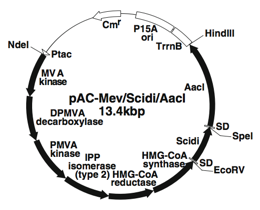
\includegraphics[width=0.5\textwidth]{aaaa.png}
  \caption{\label{fig:pac} Esquema del pl\'asmido pAC-Mev/Scidi/Aacl. Tomado de \cite{harada09b}.}
 \end{figure}


Debido a que este sistema es muy espec\'ifico a ciertas plantas, en este proyecto se busca hacerlo m\'as general, peritiendo que muchas especies de plantas se puedan proteger de una forma m\'as eficiente de los herv\'iboros sin necesidad de usar qu\'imicos insecticidas, los cu\'ales son muy nocivos para el ecosistema. De esta forma, se busca modificar a la bacteria \emph{Escherichia coli} para que produzca Bergamoteno cuando ella detecte da\~no por herbivor\'ia. Este proyecto presenta el desafio de controlar la producci\'on de Farnesil pirofosfato (FPP) porque es t\'oxico para \emph{E. coli}, adem\'as se busca optimizar la producci\'on de bergamoteno de tal forma que no sea da\~nino para la planta a largo plazo.\\

Se utiliz\'o E. coli porque el pl\'asmido pAC-Mev/Scidi/Aacl, que es el componente principal del circuito, ha sido probado \'unicamente en E. coli \cite{harada09b}. Adem\'as, aplicarlo en bacterias que crezcan de manera m\'as \'optima junto a las plantas podr\'ia generar problemas relacionados con el control de las mismas.

\section{Modelo}
\label{sec:model}
\subsection{Dise\~no}

Para el siguiente modelo cosideramos 2 partes. La primera se refiere a la produce la enzima \emph{Bergamoteno sintetasa} (E en la figura \ref{fig:Circuit}). La otra parte requiere del pl\'asmido \emph{pAC-Mev/Scidi/Aacl}, que sintetiza las enzimas necesarias para llevar \emph{Acetil CoA} a FPP. En el modelo condensamos todos los procesos enzim\'aticos que est\'an mediados por las enzimas para las que el pl\'asmido codifica en un s\'olo proceso enzim\'atico donde el sustrato A presente en la c\'elula reacciona con la enzima Z producida por el pl\'asmido para producir FPP(F en la figura \ref{fig:Circuit}). Ambas partes tienen un promotor activado por la se\~nal de da\~no. Naturalmente el sistema detecta sustancias que producen los herb\'ivoros, sin embargo, dada la dificultad para encontrar promotores activados por sustancias tan espec\'ificas, se utilizar\'a el promotor \emph{ABRA} que se encuentra en organismos vegetales y est\'a asociado a la recepci\'on y señalizaci\'on de \'acido absc\'icico (ABA). Adem\'as, el circuito del pl\'asmido presenta un sitio de inhibici\'on de LacI, el cual es producido por este mismo circuito para generar un feedback negativo. De esta manera, se busca regular la producci\'on de la enzima Z, y as\'i limitar la concentraci\'on de FPP.\\

\begin{figure}[H]
  \centering
  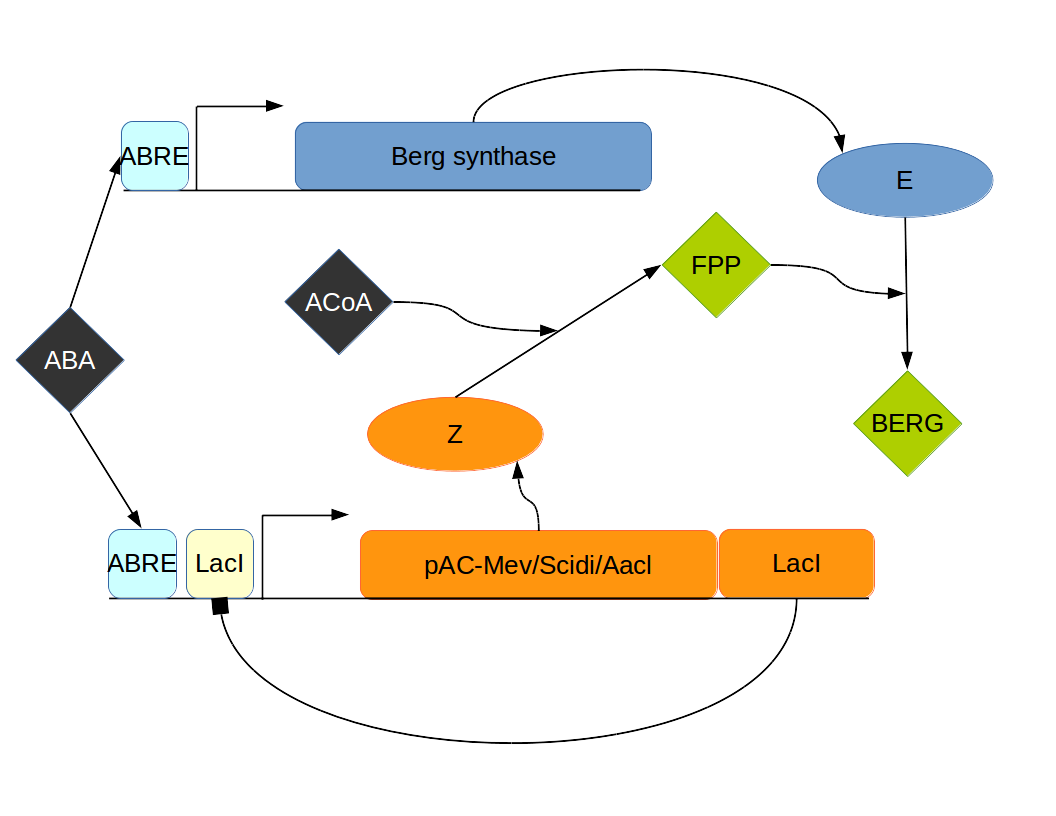
\includegraphics[width=0.5\textwidth]{Circuit.png}
  \caption{\label{fig:Circuit} Interconecciones entre los genes que se van a usar en el modelo.}
\end{figure}

El modelo que se explicar\'a a continuaci\'on tiene como objetivo principal buscar c\'omo se puede producir bergamoteno eficientemente manteniendo al m\'inimo posible la concentraciones de FPP en las c\'elulas.

\subsection{Ecuaciones de Hill}

Se model\'o la parte transcripcional como se ha hecho en clase y est\'a explicado en \cite{alon06}. Consideramos que el ADN total del gen a transcribir $\text{D}_{\text{T}}$ es constante, es decir:

\begin{equation} \label{eq:D_T}
[\text{D}_{\text{T}}]=[\text{D}]+[\text{DS}]+[\text{DI}]+[\text{DIS}],
\end{equation}

Donde $[\text{D}]$ representa el ADN libre, $[\text{DIS}]$ el ADN unido tanto al represor I como al activador S, $[\text{DS}]$ el unido al activador, y $[\text{DI}]$ el unido al represor.\\

Para realizar balance detallado se consideraron las siguientes ecuaciones qu\'imicas, las cuales son equivalentes al diagrama del inicio  de la primera tarea del curso.

\begin{align}
\ce{[D] + [S]} &\ce{<=>[\ce{k_{S+}}][\ce{k_{S-}}] [DS]}, \label{eq:rchem1}\\ 
\ce{[D] + [I]} &\ce{<=>[\ce{k_{I+}}][\ce{k_{I-}}] [DI]}, \label{eq:rchem2}\\
\ce{[DS] + [I]} &\ce{ <=>[\ce{k_{I+}}][\ce{k_{I-}}] [DIS]}, \label{eq:rchem3}\\ 
\ce{[DI] + [S]} &\ce{<=>[\ce{k_{S+}}][\ce{k_{S-}}] [DIS]}. \label{eq:rchem4}
\end{align}

Donde las $k$ son las constantes de las respectivas reacciones y se define la constante de disociaci\'on como $K = \frac{k_-}{k_+}$ \cite{alon06}. Seg\'un las ecuaciones qu\'imicas podemos plantear las ecuaciones diferenciales. Al evaluar tiempos mucho mayores a los tiempos en los que ocurre la uni\'on entre el ADN y los factores de transcripci\'on es v\'alido suponer que se ha alcanzado el estado estacionario, obteniendo entonces de las ecuaciones anteriores:

\begin{equation}
\label{eq:Dss}
\dot{[\text{D}]}=0=-k_{S+}[\text{D}][\text{S}]+k_{S-}[\text{DS}]=-k_{I+}[\text{D}][\text{I}]+k_{I-}[\text{DI}],
\end{equation}

De donde se tiene que:

\begin{equation}
\label{eq:K1}
[D][S]=K_S[DS], \quad [D][I]=K_I[DI] 
\end{equation}

Ahora se busca hallar la raz\'on entre el ADN en los distintos estados (dados por la ecuaci\'on \ref{eq:D_T}), se realizar\'a detalladamente para $[DS]$. De la ecuaci\'on \ref{eq:K1} se obtiene:

\begin{equation}
\label{eq:DS}
[D] = \frac{K_S}{S}[DS], \quad [DIS] = \frac{I}{K_I}[DS], \quad [DI]=\frac{K_S}{S}[DIS]=\frac{K_S}{S}\frac{I}{K_I}[DS],
\end{equation}

Para incluir los coeficientes de Hill en el modelo, se realiza el mismo an\'alisis pero considerando la posibilidad de que varias mol\'eculas de los factores de transcripci\'on pueden unirse al ADN, siguiendo el procedimiento del ap\'endice A.2 de \cite{alon06} obtenemos un resultado similar a la ec. \ref{eq:DS}, pero con las fracciones dependientes de S e I elevadas a los coeficientes de Hill $n_S$ y $n_I$, respectivamente. Por lo tanto al reemplazar esto en la ec. \ref{eq:D_T} y reorganizando se tiene que:

\begin{equation}
\frac{[DS]}{[D_T]} = \frac{1}{\left( \frac{K_S}{S} \right)^{n_S} + \left( \frac{I}{K_I} \right)^{n_I} \left( \frac{K_S}{S} \right)^{n_S} + 1 + \left( \frac{I}{K_I} \right)^{n_I}},
\end{equation}

La expresi\'on anterior representa la fracci\'on de ADN ligado a $S$ que hay en equilibrio, al considerar un tiempo suficientemente largo para que ocurran muchos eventos de uni\'on y disociaci\'on de los factores de transcripci\'on esto se puede interpretar como la probabilidad de que el ADN se encuentre en este estado y por lo tanto que la transcripci\'on se d\'e en \'el. As\'i, al multiplicar por la fuerza del promotor $\beta$ obtenemos la tasa de transcripci\'on en dicho estado del ADN.\\

De la misma manera se pueden realizar el an\'alisis para $[DI]$, $[D]$ y $[DIS]$ para obtener las tasas de transcripci\'on en cada uno de los estados. La tasa total es la suma de todas las tasas, donde adem\'as se toma la tasa correspondiente al ADN libre como una constante $\alpha$ correspondiente a la transcripci\'on basal. Tambi\'en se sigue un procedimiento similar para hallar la tasa de producci\'on de $r_E$, que es mucho m\'as sencillo pues s\'olo hay un promotor. Se incluye un t\'ermino de degradaci\'on $\gamma$ tanto de ARN como de prote\'inas y se incluye tambi\'en una tasa de creaci\'on de prote\'inas $k_P$ que tomaremos como constante y se determinar\'a seg\'un el RBS.\\

Las ecuaciones que se obtienen son las siguientes:

\begin{multline}
\label{eq:rZ}
\dot{r_Z}(t) = 
\alpha_{IS}
+ \frac{\beta_{IS_I}}{\left( \frac{K_I}{I} \right)^{n_I} + 1 + \left( \frac{S}{K_S} \right)^{n_S} \left( \frac{K_I}{I} \right)^{n_I} + \left( \frac{S}{K_S} \right)^{n_S}}\\
+ \frac{\beta_{IS_S}}{\left( \frac{K_S}{S} \right)^{n_S} + \left( \frac{I}{K_I} \right)^{n_I} \left( \frac{K_S}{S} \right)^{n_S} + 1 + \left( \frac{I}{K_I} \right)^{n_I}}
+ \frac{\beta_{IS_{IS}}}{\left( \frac{K_I}{I} \right)^{n_I} \left( \frac{K_S}{S} \right)^{n_S} + \left( \frac{K_S}{S} \right)^{n_S} + \left( \frac{K_I}{I} \right)^{n_I} + 1}
- \gamma_{r_Z} r_Z
\end{multline}

\begin{equation}
\label{eq:Z}
\dot{Z}(t) = k_Z r_Z - \gamma_Z Z
\end{equation}

\begin{multline}
\label{eq:rI}
\dot{r_I}(t) = 
\alpha_{IS}
+ \frac{\beta_{IS_I}}{\left( \frac{K_I}{I} \right)^{n_I} + 1 + \left( \frac{S}{K_S} \right)^{n_S} \left( \frac{K_I}{I} \right)^{n_I} + \left( \frac{S}{K_S} \right)^{n_S}}\\
+ \frac{\beta_{IS_S}}{\left( \frac{K_S}{S} \right)^{n_S} + \left( \frac{I}{K_I} \right)^{n_I} \left( \frac{K_S}{S} \right)^{n_S} + 1 + \left( \frac{I}{K_I} \right)^{n_I}}
+ \frac{\beta_{IS_{IS}}}{\left( \frac{K_I}{I} \right)^{n_I} \left( \frac{K_S}{S} \right)^{n_S} + \left( \frac{K_S}{S} \right)^{n_S} + \left( \frac{K_I}{I} \right)^{n_I} + 1}
- \gamma_{r_I} r_I
\end{multline}

\begin{equation}
\label{eq:I}
\dot{I}(t) = k_I r_I - \gamma_I I
\end{equation}

\begin{equation}
\label{eq:r_E}
\dot{r_E}(t) = \alpha_S + \frac{\beta_S}{1+ \left( \frac{K_S}{S}\right)^{n_S}} - \gamma_{r_E} r_E\\
\end{equation}

\begin{equation}
\label{eq:E}
\dot{E}(t) = k_E r_E - \gamma_EE
\end{equation}

\subsection{Reacciones enzim\'aticas}

Seg\'un la figura \ref{fig:Circuit}, las ecuaciones qu\'imicas de las reacciones entre enzima y sustrato son las siguientes

\begin{align}
\ce{[Z] + [A]} &\ce{<=>[\ce{\hat{k}_+}][\ce{\hat{k}_-}] [ZA] ->[\ce{\hat{k}_{cat}}] [Z] + [F]}, \label{eq:echem1}\\
\ce{[E] + [F]} &\ce{<=>[\ce{k_+}][\ce{k_-}] [EF] ->[\ce{k_{cat}}] [E] + [B]}, \label{eq:echem2}
\end{align}

donde [Z] y [E] son las enzimas que proceden del pl\'asmido y la bergamoteno sintetasa, respectivamente. [F] y [B] corresponden a FPP y el bergamoteno. Con las ecuaciones \ref{eq:echem1} y \ref{eq:echem2}, se obtubieron las ecuaciones diferenciales para el FPP y el Bergamoteno, siguiendo el siguiente razonamiento.\\

Debido a que el Acetil CoA, el sustrato de la enzima que produce FPP, proviene del metabolismo constante de la bacteria, se puede suponer que su concentraci\'on $[A]$ es constante y elevada. Por lo tanto, para la producci\'on de FPP habr\'a un t\'ermino positivo que sigue las ecuaciones de Michaelis-Menten.\\

Por otra parte, debido a que el FPP est\'a siendo consumido a la vez para producir Bergamoteno, se requiere un t\'ermino negativo en la ecuaci\'on diferencial que ilustre este proceso. Sin embargo, se usa la aproximaci\'on de la ecuaci\'on de velocidad cuadr\'atica ilustrado en \cite{chemwiki1}. Esta ecuaci\'on es v\'alida cuando la concentraci\'on de sustrato no es constante y es similar a la concentraci\'on de la enzima que cataliza dicho sustrato \cite{chemwiki1}. Dicho esto, las ecuaciones que se usar\'an son

\begin{eqnarray}
\dot{F} &=& \frac{K_{\text{cat1}}[Z][A]}{K_{\text{M1}}+[A]} - K_{\text{cat2}}\frac{J-\sqrt{J^2-4[E][F]}}{2} \label{eq:DiffF}\\
\dot{B} &=& K_{\text{cat2}}\frac{J-\sqrt{J^2-4[E][F]}}{2} - \gamma_B [B] \label{eq:DiffB}\\
\text{Donde} && J=[E]+[F]+K_{\text{M2}} \nonumber
\end{eqnarray}

Y $K_{M1}$, $K_{\text{cat}1}$, $K_{M2}$, $K_{\text{cat}2}$, son las constantes de las enzimas del pl\'asmido y de la bergamoteno sintetasa, respectivamente. $\gamma_B$ es el t\'ermino introducido por el decaimiento del Bergamoteno debido a la difusi\'on y divisi\'on celular. Este t\'ermino no es inclu\'ido en la ecuaci\'on para F pues esta sustancia es utilizada en otra reacci\'on enzim\'atica que ocurre mucho m\'as r\'apido que el tiempo de degradaci\'on de las prote\'inas.\\

Las ecuaciones diferenciales para F y B (\ref{eq:DiffF} y \ref{eq:DiffB}) dependen de las cantidades calculadas con el modelo estoc\'astico para la producci\'on de las enzimas, estas cantidades siguen la din\'amica ilustrada en la secci\'on anterior.\\

Las ecuaciones \ref{eq:rZ} - \ref{eq:E}, \ref{eq:DiffF} y \ref{eq:DiffB}, junto con las condiciones iniciales para cada una, constituyen el sistema de ecuaciones que ser\'a simulado mediante los programas.

\subsection{Par\'ametros}

En la tabla \ref{tab:1} est\'an listados los par\'ametros del modelo.

\begin{table}[H]
\centering
\begin{tabular}{c c c c c} 
 \hline
 S\'imbolo & Valor & Unidades & Descripci\'on & Ref. \\
 \hline\hline
 W & 1791/RFP & - & Mutaci\'on en el promotor constitutivo & BBa\_J23113 \\
 $\alpha_S$ & $1.53/W$ & - & Actividad basal de S & \cite{kelly09}  \\ 
 $\beta_S$ & $51.2 \alpha_S$ & - &  Actividad de S con ABA & \cite{hobo99} \\
 $\alpha_{RS}$ & $1.53/W$ & - & Actividad basal de RS & \cite{kelly09} \\
 $\beta_{RS_R}$ & $\alpha_{RS}/620$ & - & Actividad de RS con LacI & \cite{lutz97}\\
 $\beta_{RS_S}$ & $51.2 \alpha_{RS}$ & - & Actividad de  RS con ABA & \cite{hobo99} \\
 $\beta_{RS_RS}$ & $\beta_{RS_R}$ & - & Actividad de RS con ABA y LacI & \cite{lutz97} \\
 $K_S$ & * &  & Constante de disociaci\'on del ABA-ABRE &  \\
 $n_S$ & * &  & Coeficiente de Hill de S & \\
 $k_E$ & * &  & Tasa de traducci\'on de E &   \\
 $K_R$ & $8*10^{-4}$ & mM & Constante de disociaci\'on de LacI & \cite{basu05} \\
 $n_R$ & 1 & - & Coeficiente de Hill de LacI & \cite{kalisky07}\\
 $k_R$ & * & & Tasa de traducci\'on de R & \\
 $\gamma_R$ & * & & Tasa de degradaci\'on de la enzima Z & \\
 $\gamma_E$ & 1/30 & $min^{-1}$ & Tasa de degradaci\'on del ARN (de E y R) & \\
 $K_{MBerg}$ & 0.0014 & $mM$ & Constante de MM para enzima E & \cite{jones11} \\
 $K_{CBerg}$ & 0.34 & $s^{-1}$ & Turnover para enzima E & \cite{jones11} \\
 $K_{MFpp}$ & 0.0048 & $mM$ & Constante de MM para enzima Z & \cite{kittleman07} \\
 $K_{CFpp}$ & 0.34 & $s^{-1}$ & Turnover para enzima Z & \cite{kittleman07} \\
 \hline
\end{tabular}
\caption{Par\'ametros del modelo. S hace referencia al promotor \emph{ABRA} individual y RS al promotor \emph{ABRA} con el sitio de \emph{lacI}. Las tasas de degradaci\'on $\gamma$ se tomaron iguales en todos los casos. Los se\~nalados con * no fueron encontrados (ver secci\'on \ref{sens}).}
\label{tab:1}
\end{table}

\subsection{Modelos determinista y estoc\'astico}

Para realizar la simulaci\'on estoc\'astica se utiliz\'o el algoritmo de Gillespie. Si los eventos de producci\'on de ARN y prote\'inas son considerados separadamente se tendr\'ian 8 eventos, lo cual tomar\'ia mucho tiempo en ejecutar. Por lo tanto, se realiz\'o el algoritmo con r\'afagas de prote\'inas, de tal forma que al evento de producirse un RNA, se producen $\frac{k_P}{\gamma_r}$ prote\'inas. Esto es lo que corresponde al promedio de prote\'inas que se pueden traducir de un RNA durante su tiempo de vida.\\

Por otra parte, las escalas de tiempo a las que ocurren las reacciones enzim\'aticas son mucho menores a las de la producci\'on de RNA y prote\'inas, por lo tanto los efectos del ruido son despreciables en ellas y por lo tanto se pueden resolver de manera determinista. Se utiliz\'o en este caso el m\'etodo Runge-Kutta de Cuarto Orden.\\

En programa fu\'e realizado utilizado IPython notebook, se puede ver el c\'odigo fuente en \url{https://github.com/gutiloluis/Insecticida/blob/master/Sensibilidad.ipynb}. En el repositorio donde se encuentra este programa est\'a tambi\'en todo lo realizado en el proceso de desarrollo del programa.

\subsection{An\'alisis de sensibilidad}
\label{sens}
Se realiz\'o un an\'alisis de sensibilidad usando las constantes que no se conocen. \'Estas se pueden dividir en 2 grupos, $W$ y $\gamma_R$ que son manipulables y $K_S$, $n_S$, $k_E$ y $k_R$ que son las que queremos optimizar. A partir de esto, se seleccionaron 3 niveles distintos para $W$ y $\gamma_R$, y 4 niveles posibles para las dem\'as. Para escoger el r\'ango \'optimo, se estableci\'o que la concentraci\'on de FPP m\'axima no pod\'ia superar los $0.0004 $ mM y que el nivel de bergamoteno prodicido fuera el m\'aximo. Esto se justifica porque no queremos una cantidad de FPP que llegue a ser t\'oxica muy r\'apidamente, y queremos la mayor cantidad posible de bergamoteno.\\

\begin{figure}[H]
  \begin{subfigure}[b]{0.5\textwidth}
  	\centering
  	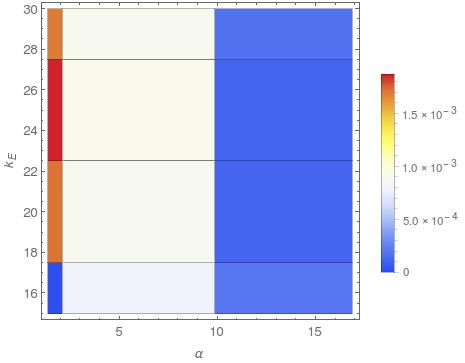
\includegraphics[width=\textwidth]{alpha-kE.jpeg}
  	\caption{\label{fig:alpha-kE} Barrido para $\alpha$ y $k_E$.}
  \end{subfigure}
  \begin{subfigure}[b]{0.5\textwidth}
  	\centering
  	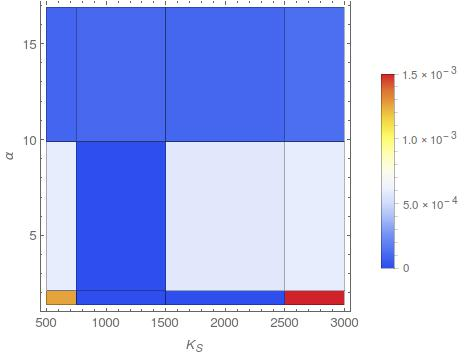
\includegraphics[width=\textwidth]{alpha-KS.jpeg}
  	\caption{\label{fig:alpha-kS} Barrido para $\alpha$ y $K_S$.}
  \end{subfigure}
    
  \begin{subfigure}[b]{0.5\textwidth}
	\centering
  	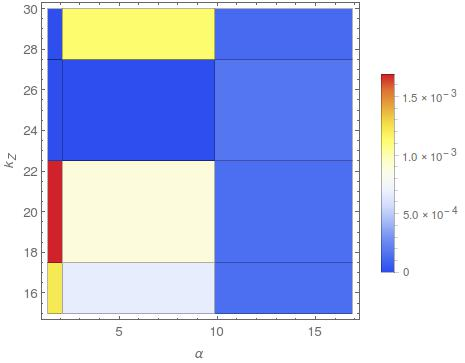
\includegraphics[width=\textwidth]{alpha-kz.jpeg}
  	\caption{\label{fig:alpha-kz} Barrido para $\alpha$ y $k_Z$.}
  \end{subfigure}  
  \begin{subfigure}[b]{0.5\textwidth}
  	\centering
  	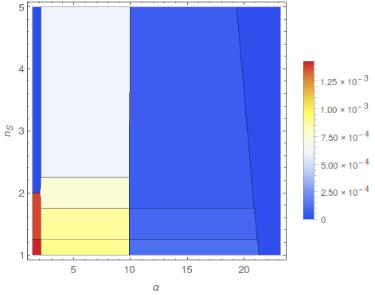
\includegraphics[width=\textwidth]{alpha-nS.jpeg}
  	\caption{\label{fig:alpha-nS} Barrido para $\alpha$ y $n_S$.}
  \end{subfigure}  
\caption{\label{fig:alpha} an\'alisis para $\alpha$} 
\end{figure}

\begin{figure}[H]
	\begin{subfigure}[b]{0.5\textwidth}
  		\centering
  		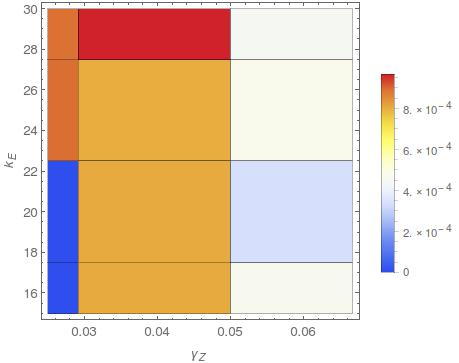
\includegraphics[width=\textwidth]{gammaZ-kE.jpeg}
  		\caption{\label{fig:gammaZ-kE} Barrido para $\gamma_Z$ y $k_E$.}
  	\end{subfigure}
	\begin{subfigure}[b]{0.5\textwidth}
		\centering
  		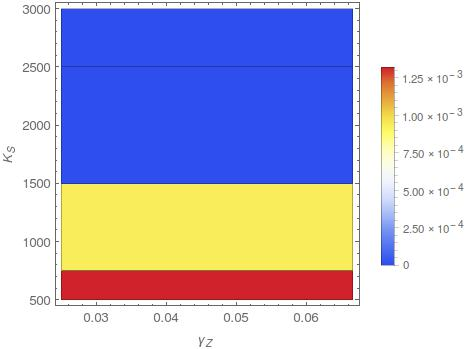
\includegraphics[width=\textwidth]{gammaZ-KS.jpeg}
		\caption{\label{fig:gammaZ-KS} Barrido para $\gamma_Z$ y $K_S$.}
  	\end{subfigure} 	
  	
  	\begin{subfigure}[b]{0.5\textwidth}
		\centering
		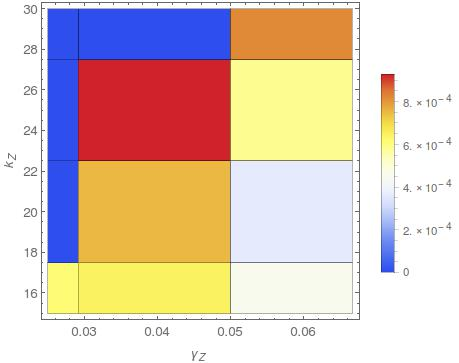
\includegraphics[width=\textwidth]{gammaZ-kZ.jpeg}
		\caption{\label{fig:gammaZ-kZ} Barrido para $\gamma_Z$ y $k_Z$.}
  	\end{subfigure} 	
  		\begin{subfigure}[b]{0.5\textwidth}
		\centering
		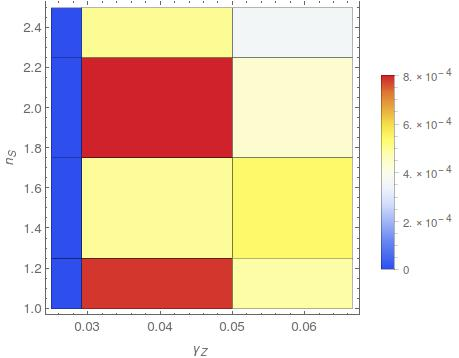
\includegraphics[width=\textwidth]{gammaZ-nS.jpeg}
		\caption{\label{fig:gammaZ-nS} Barrido para $\gamma_Z$ y $n_S$.}
  	\end{subfigure} 	
 \caption{\label{fig:gammaZ} an\'alisis para $\gamma _Z$}	
 \end{figure}

Se puede observar que para valores de $W = 6 $ (ver fig.\ref{fig:alpha}) y de $\gamma _Z = 0.04$ (ver fig.\ref{fig:gammaZ}) se obtienen los valores m\'as estables para las diferentes combinaciones de las dem\'as constantes. Hay que recordar que $W$ est\'a relacionado inversamente con la producci\'on basal de RNA tanto para los circuitos del pl\'asmido como para los de la enzima del bergamoteno, por lo que un valor como este significar\'ia una mutaci\'on no muy deleterea en el sitio del promotor. Mientras que para $\gamma _Z$ se est\'a cerca del valor promedio de degradaci\'on de una prote\'ina.

\section{M\'etodos Experimentales}

Para obtener el sistema propuesto, es necesario ensamblar dos regiones promotoras/operadoras, un represor, el inserto proveniente del plásmido pAC-Mev \cite{harada09a}, y la secuencia codificante para la bergamoteno sintasa. Este ensamblaje se realizará siguiendo la estrategia del 3A-Assembly utilizada en iGEM \cite{igem}, en la cual se utilizan las enzimas de restricción EcoRI, SpeI, XbaI y PstI para ensamblar las partes de manera secuencial. Por esta razón, todas las partes utilizadas deben estar flaqueadas por estos sitios de restricción.\\

Los promotores son complejos y contienen regiones regulatorias en diferentes ubicaciones, de manera que lo más eficiente es pedir la síntesis de estos oligonucleótidos. Para utilizar el fragmento que contiene las enzimas de la vía que va desde el acetil-CoA hasta el FPP, se espera obtener el plásmido pAC-Mev y digerirlo con las enzimas NdeI y EcoRV. El fragmento se clonaría en un plásmido pUC19 para obtener los sitios de restricción de XbaI y SpeI. El fragmento correspondiente a la bergamoteno sintasa se va a amplificar a partir del árbol de sándalo (\emph{Santalum album}), utilizando primers a los cuales se les añadió los sitios de restricción anteriormente mencionados (ver Anexo). Durante el diseño de los primers se tuvo en cuenta la estabilidad de posibles estructuras secundarias y de homo- y heterodímeros en la plataforma de \url{IDT.com} \cite{owczarzy08}. Finalmente, la secuencia del represor LacI, así como la del sitio de unión al ribosoma, se va a obtener a partir de la distribución de partes de iGEM, de manera que esta ya tendrá los sitios de restricción requeridos.\\

Siendo E. coli nuestro chasis final, el constructo se va a generar mediante sucesivas restricciones y ligaciones en los plásmidos pSB1C3, pSB1A3 y pAB1K3 \cite{igem} en esta bacteria. Se va a utilizar LB (Lysis Broth) como medio de cultivo, suplementado con el antibiótico de selección necesario. Se van a obtener los plásmidos por medio del kit GenElute™ HP Plasmid Miniprep Kit (Sigma) y éstos van a ser sometidos a digestión por las enzimas EcoRI y SpeI, XbaI y PstI o EcoRi y PstI, dependiendo del caso. Finalmente, se van a ligar las partes de interés en uno de los plásmidos anteriormente mencionados.\\

Cuando se tenga el constructo final en un plásmido, se va a insertar el mismo en el cromosoma de E. coli. Una buena opción para hacerlo de manera dirigida es el sistema de CRISPR-Cas, el cual ha sido altamente utilizado para la edición de genomas \cite{xie13}, es probable que sea problemática la longitud del inserto pues es de m\'as de 10 kb.

\section{Consideraciones \'Eticas}

El presente proyecto contempla la liberación al medio ambiente de bacterias modificadas genéticamente y, por lo tanto, existen diferentes riesgos que habría que evaluar. Por ejemplo, es posible que se de una transferencia horizontal de los genes insertados artificialmente. Sin embargo, el diseño propuesto se basa en la integración del sistema en el cromosoma, evitando así el uso de plásmidos cuya movilidad puede llegar a ser muy alta. Sin embargo, existe la posibilidad de encontrar eventos de transferencia horizontal de segmentos de cromosoma, por ejemplo mediada por fagos. Aunque sería poco probable que se transfiriera todo el constructo propuesto a una frecuencia tal que desencadene un cambio notable en el ambiente, las consecuencias de esta eventual perturbación podrían ser importantes y difíciles de estimar.\\

Por otro lado, es posible que las bacterias modificadas sufran mutaciones en el ambiente. Se debe tener en cuenta que es más probable que estas mutaciones generen una pérdida de función de algún gen que una ganancia de una función novedosa. Una posibilidad es que el sistema pierda su capacidad de ser inducible por la señal relacionada con herbivoría y que la producción de bergamoteno se vuelva constitutiva. Esto es poco probable, dado el alto costo metabólico que representa la síntesis de este compuesto pero, si por alguna razón el compuesto o su producción confieren alguna ventaja evolutiva, se tendrían consecuencias ambientales importantes. De hecho, el efecto de este cambio sería similar al de un mal uso del eventual producto por parte de los clientes: si no se asperja la bacteria sólo en la época en la que se espera la llegada de los herbívoros, sino de manera continua, es posible que la bacteria responda de manera no específica y se produzca suficientes cantidades de bergamoteno para atraer al depredador. Si este caso se prolonga lo suficiente, el depredador sufriría una presión de selección para dejar de acercarse a las fuentes de bergamoteno y el sistema propuesto dejaría de funcionar.

\appendix
\section{Ap\'endice: Partes}
\subsection{Promotor}

\begin{verbatim}
AGCGGAGCCCTGACAGCTAGCTCAGTCCTAGGTATAATGCTAGCATAAATGTGAGCGGATAACATTGGGTTTGT
AGCCGATAACAA
\end{verbatim}

Referencias: \cite{hobo99} \cite{lutz97}.

\subsection{LacI}

\begin{verbatim}
ATGGTGAATGTGAAACCAGTAACGTTATACGATGTCGCAGAGTATGCCGGTGTCTCTTATCAGACCGTTTCCCC
GTGGTGAACCAGGCCAGCCACGTTTCTGCGAAAACGCGGGAAAAAGTGGAAGCGGCGATGGCGGAGCTGAATTA
CATTCCCAACCGCGTGGCACAACAACTGGCGGGCAAACAGTCGTTGCTGATTGGCGTTGCCACCTCCAGTCTGG
CCCTGCACGCGCCGTCGCAAATTGTCGCGGCGATTAAATCTCGCGCCGATCAACTGGGTGCCAGCGTGGTGGTG
TCGATGGTAGAACGAAGCGGCGTCGAAGCCTGTAAAGCGGCGGTGCACAATCTTCTCGCGCAACGCGTCAGTGG
GCTGATCATTAACTATCCGCTGGATGACCAGGATGCCATTGCTGTGGAAGCTGCCTGCACTAATGTTCCGGCGT
TATTTCTTGATGTCTCTGACCAGACACCCATCAACAGTATTATTTTCTCCCATGAAGACGGTACGCGACTGGGC
GTGGAGCATCTGGTCGCATTGGGTCACCAGCAAATCGCGCTGTTAGCGGGCCCATTAAGTTCTGTCTCGGCGCG
TCTGCGTCTGGCTGGCTGGCATAAATATCTCACTCGCAATCAAATTCAGCCGATAGCGGAACGGGAAGGCGACT
GGAGTGCCATGTCCGGTTTTCAACAAACCATGCAAATGCTGAATGAGGGCATCGTTCCCACTGCGATGCTGGTT
GCCAACGATCAGATGGCGCTGGGCGCAATGCGCGCCATTACCGAGTCCGGGCTGCGCGTTGGTGCGGATATCTC
GGTAGTGGGATACGACGATACCGAAGACAGCTCATGTTATATCCCGCCGTTAACCACCATCAAACAGGATTTTC
GCCTGCTGGGGCAAACCAGCGTGGACCGCTTGCTGCAACTCTCTCAGGGCCAGGCGGTGAAGGGCAATCAGCTG
TTGCCCGTCTCACTGGTGAAAAGAAAAACCACCCTGGCGCCCAATACGCAAACCGCCTCTCCCCGCGCGTTGGC
CGATTCATTAATGCAGCTGGCACGACAGGTTTCCCGACTGGAAAGCGGGCAGGCTGCAAACGACGAAAACTACG
CTTTAGTAGTTAATAACTCTGATAGT
\end{verbatim}

Referencias: \cite{igemP}

\subsection{pAC-Mev}

Referencias: En \cite{harada09a}, se incluyen las secuencias de los primers de los genes que contiene el pl\'asmido.

\subsection{Bergamoteno sintasa}

\begin{verbatim}
ATGGATTCTTCCACCGCCACCGCCATGACAGCTCCATTCATTGATCCTACTGATCATGTGAATCTCAAAACTGA
TACGGATGCCTCAGAGAATCGAAGGATGGGAAATTATAAACCCAGCATTTGGAATTATGATTTTTTACAATCAC
TTGCAACTCATCACAATATTGTGGAAGAGAGGCATCTAAAGCTAGCTGAGAAGCTGAAGGGCCAAGTGAAGTTT
ATGTTTGGGGCACCAATGGAGCCGTTAGCAAAGCTGGAGCTTGTGGATGTGGTTCAAAGGCTTGGGCTAAACCA
CCTATTTGAGACAGAGATCAAGGAAGCGCTGTTTAGTATTTACAAGGATGGGAGCAATGGATGGTGGTTTGGCC
ACCTTCATGCGACATCTCTCCGATTTAGGCTGCTACGACAGTGTGGGCTTTTTATTCCCCAAGATGTGTTTAAA
ACGTTCCAAAACAAGACTGGGGAATTTGATATGAAACTTTGTGACAACGTAAAAGGGCTGCTGAGCTTATATGA
AGCTTCATACTTGGGATGGAGGGTGAAAACATCCTAGATGAAGCCAAGGCCTTCACCACCAAGTGCTTGAAAAG
TGCATGGGAAAATATATCCGAAAAGTGGTTAGCCAAAAGAGTGAAGCATGCATTGGCTTTGCCTTTGCATTGGA
GAGTCCCTCGAATCGAAGCTAGATGGTTCATTGAGGCATATGAGCAAGAAGCGAATATGAACCCAACACTACTC
AAACTCGCAAAATTAGACTTTAATATGGTGCAATCAATTCATCAGAAAGAGATTGGGGAATTAGCAAGGTGGTG
GGTGACTACTGGCTTGGATAAGTTAGCCTTTGCAGGAATAATTTACTGCAGAGCTATATGTGGAGCTGCGCGAT
TGCTTCCGACCCGAAGTTCAAACTTGCTAGAGAAACTATTGTCGAAATCGGAAGTGTACTCACAGTTGTTGACG
ATGGATATGACGTCTATGGTTCAATCGACGAACTTGATCTCTACACAAGCTCCGTTGAAAGGTGGAGCTGTGTG
GAAATTGACAAGTTGCCAAACACGTTAAAATTAATTTTTATGTCTATGTTCAACAAGACCAATGAGGTTGGCCT
TCGAGTCCAGCATGAGCGAGGCTACAATAGCATCCCTACTTTTATCAAAGCGTGGGTTGAACAGTGTAAATCAT
ACCAGAAAGAAGCAAGATGGTTCCACGGGGGACACACGCCTCCATTGGAAGAATATAGCTTGAATGGACTTGTT
TCCATAGGATTCCCTCTCTTGTTAATCACGGGCTACGTGGCAATCGCTGAGAACGAGGCTGCACTGGATAAAGT
GCACCCCCTTCCTGATCTTCTGCACTACTCCTCCCTCCTTAGTCGCCTCATCAATGATATAGGAACGTCTCCGG
ATGAGATGGCAAGAGGCGATAATCTGAAGTCAATCCATTGTTACATGAACGAAACTGGGGCTTCCGAGGAAGTT
GCTCGTGAGCACATAAAGGGAGTAATCGAGGAGAATTGGAAAATACTGAATCAGTGCTGCTTTGATCAATCTCA
GTTTCAGGAGCCTTTTATAACCTTCAATTTGAACTCTGTTCGAGGGTCTCATTTCTTCTATGAATTTGGGGATG
GCTTTGGGGTGACGGATAGCTGGACAAAGGTTGATATGAAGTCCGTTTTGATCGACCCTATTCCTCTCGGCGAG
GAGTAG
\end{verbatim}

Referencias: GenBank: HQ343276.

\subsection{RBS}

\begin{verbatim}
AAAGAGGAGAAA
\end{verbatim}

Referencias: \cite{igemP}

\subsection{BergF}

\begin{verbatim}
GTTTCTTCGAATTCGCGGCCGCTTCTAGAGATGGATTCTTCCACCGCCA
\end{verbatim}

\subsection{BerR}

\begin{verbatim}
GTTTCTTCCTGCAGCGGCCGCTACTAGTACTACTCCTCGCCGAGAGGAATA
\end{verbatim}

\bibliographystyle{plain}
\bibliography{written.bib}

\end{document}
